\documentclass{scrartcl}
\usepackage[mathletters]{ucs}
\usepackage[utf8x]{inputenc}
\usepackage{amssymb}
\usepackage{amsmath}
\usepackage[usenames]{color}
\usepackage{hyperref}
\usepackage{wasysym}
\usepackage{graphicx}
\usepackage[normalem]{ulem}
\usepackage{enumerate}

\usepackage{listings}

\lstset{ %
basicstyle=\footnotesize,       % the size of the fonts that are used for the code
showspaces=false,               % show spaces adding particular underscores
showstringspaces=false,         % underline spaces within strings
showtabs=false,                 % show tabs within strings adding particular underscores
frame=single,                   % adds a frame around the code
tabsize=2,                      % sets default tabsize to 2 spaces
breaklines=true,                % sets automatic line breaking
breakatwhitespace=false,        % sets if automatic breaks should only happen at whitespace
}


\title{1 camera position side}
\date{dinsdag 08 december 2020}
\author{}

\begin{document}

\maketitle

		\section{1 camera position side}

Created woensdag 11 november 2020



\subsection{Camera position on the side}

Taken on the first 4 plates of batch 04 with red lighting only from the adressable led strips. 



1st light position is made with a setup with two led strips where one image is taken for every set of two led lights. 

output is bad. Reflection angle wasn't good. 

Results saved in next directory

/Users/larsdepauw/Documents/Lars.nosync/Documents/School/1Ma ing/Masterproef/Images/dataset/First\_automated/camera\_zijkant\_dual\_ledstrip



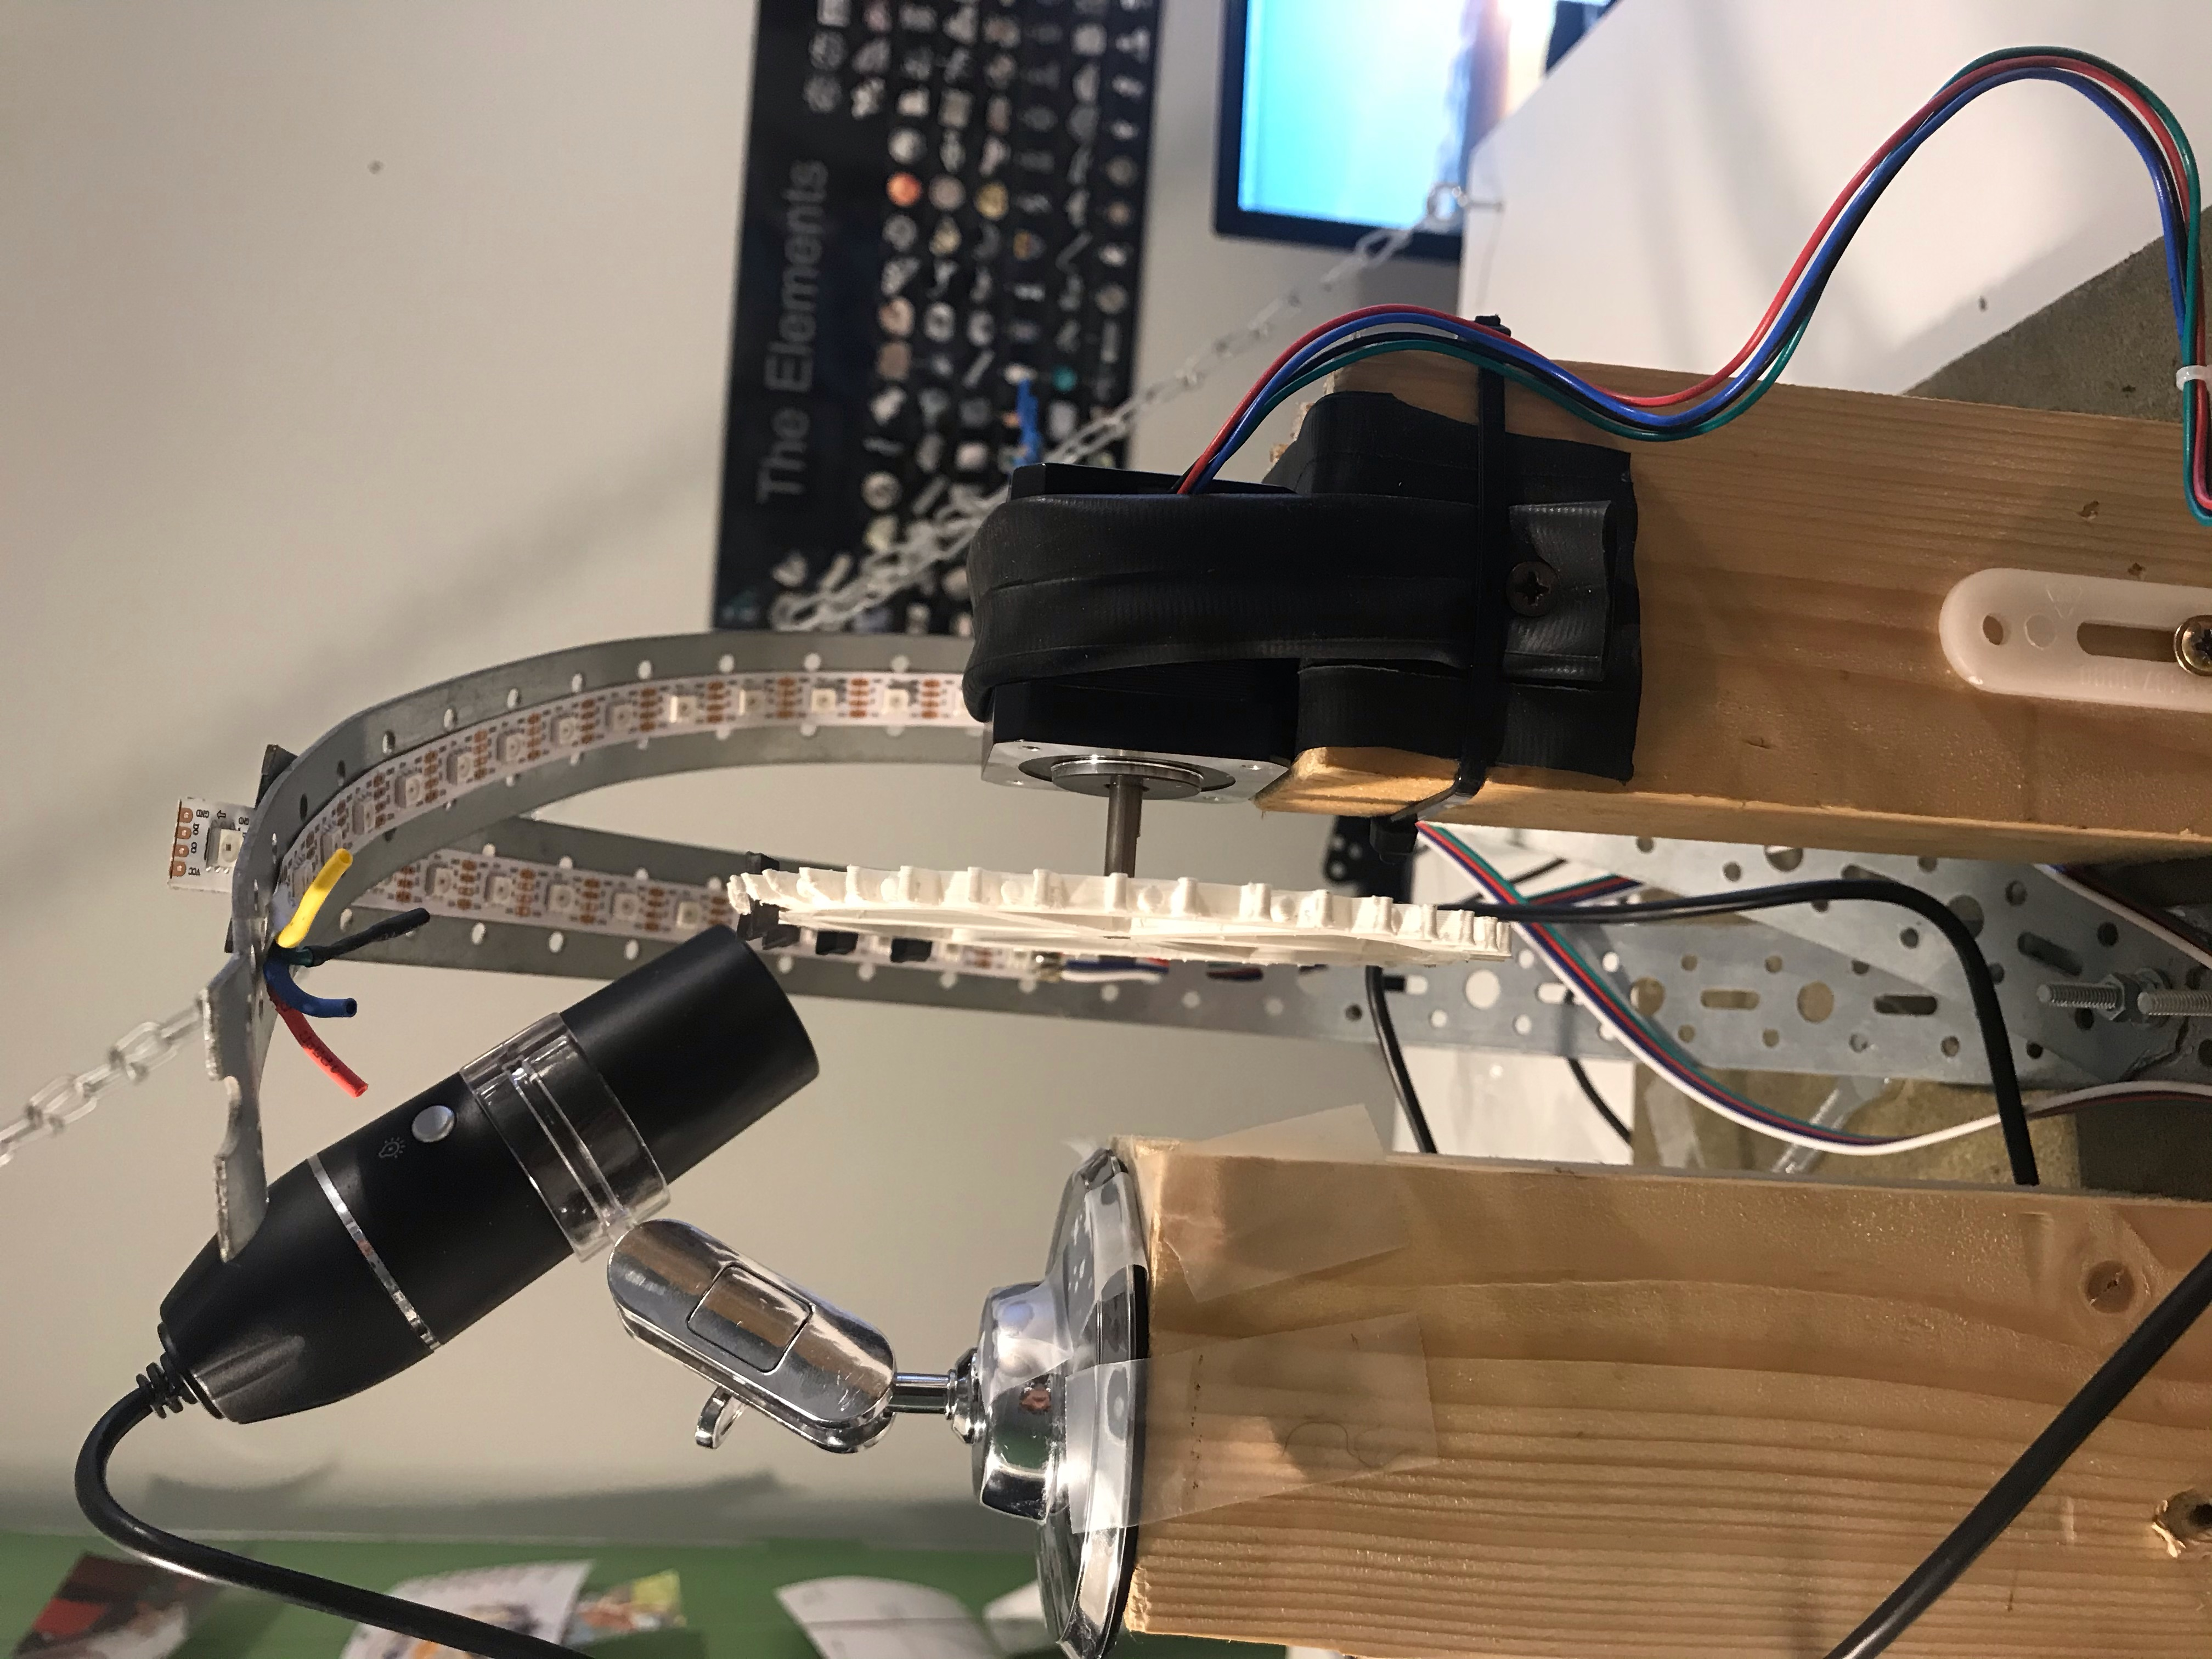
\includegraphics[width=4.166667in, keepaspectratio=true]{./1_camera_position_side/achter2.jpeg}



The images that where taken with this setup are found here:

Due to the problems with the arduino communications described \href{../../../../Code/Problems/arduino_loop_time.tex}{here} the first dataset wasn't successfull because the leds didn't turn on when the photo's where taken. So the results are all black pictures with al little shadow of the insert caused by the polluting light. 



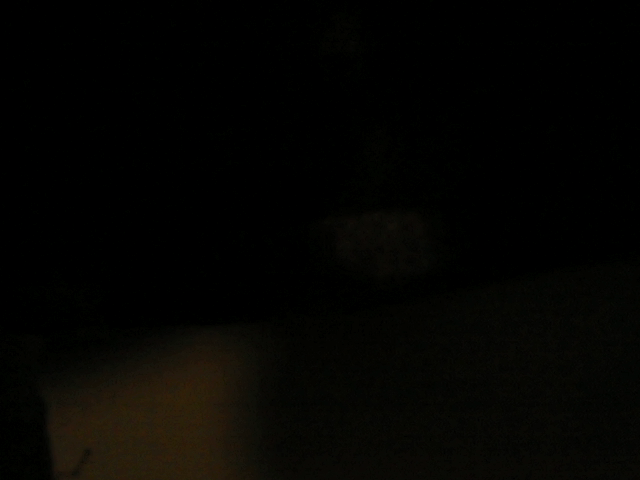
\includegraphics[width=4.166667in, keepaspectratio=true]{./1_camera_position_side/p3_l6_black.png}



\subsection{Camera position on the side take two}



A delay was entered before sending a command to the arduino to provide the wanted lighting conditions. Although this was a very long process the results are way better than the ones from the first take on this camera setup. 



The same setup was used with the camera in the same position. For red led only the following image is the result.



The leds shown here leds 8 through 10. There is a nice lighting of every part of the wear

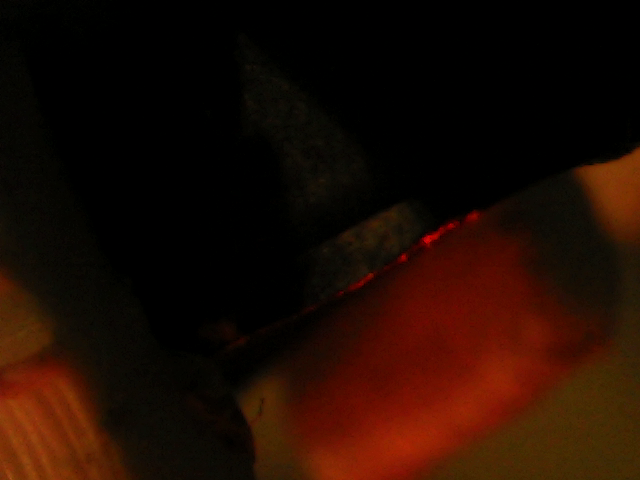
\includegraphics[width=3.125000in, keepaspectratio=true]{./1_camera_position_side/p3_l8.png}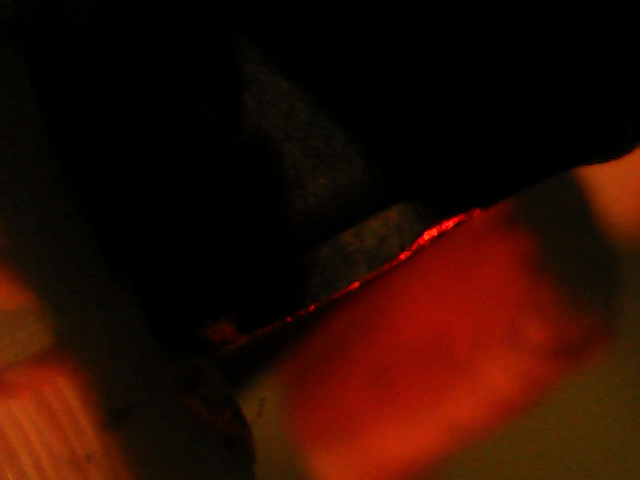
\includegraphics[width=3.125000in, keepaspectratio=true]{./1_camera_position_side/p3_l9.png}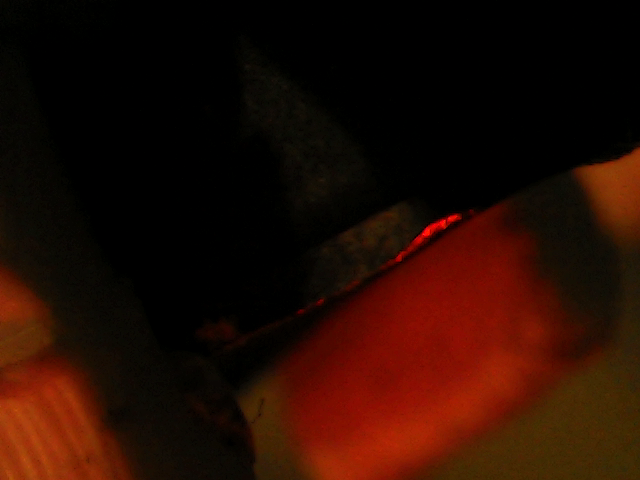
\includegraphics[width=3.125000in, keepaspectratio=true]{./1_camera_position_side/p3_l10.png}



This lightens the worn area very good. Although th ebackground is lighted as well and makes it harder to only see the worn area. On this we can build the first dataset. 

Next the \href{./2_camera_position_top.tex}{top view} was tested 



\end{document}
